\subsection{Helium Entrainment}

In most models run, during Si-burning a number of shells are merged, creating a new shell which $^{4}He$ is drawn into over time.

This is illustrated in Figure \ref{fig:HeMerger_Abundance}, where $^{40}$Ca and $^{28}$Si are drawn up whilst $^{20}Ne$ and $^{24}$Mg are drawn to deeper regions at $\log_{10}\left(\text{time to core collapse}\right) \sim -3.1$. The similar outcome of models using different mixing theories suggests the change does not qualitatively effect the outcome of this event, even given the short timescales for burning at this point. 

\begin{figure*}[t]
\begin{center}
    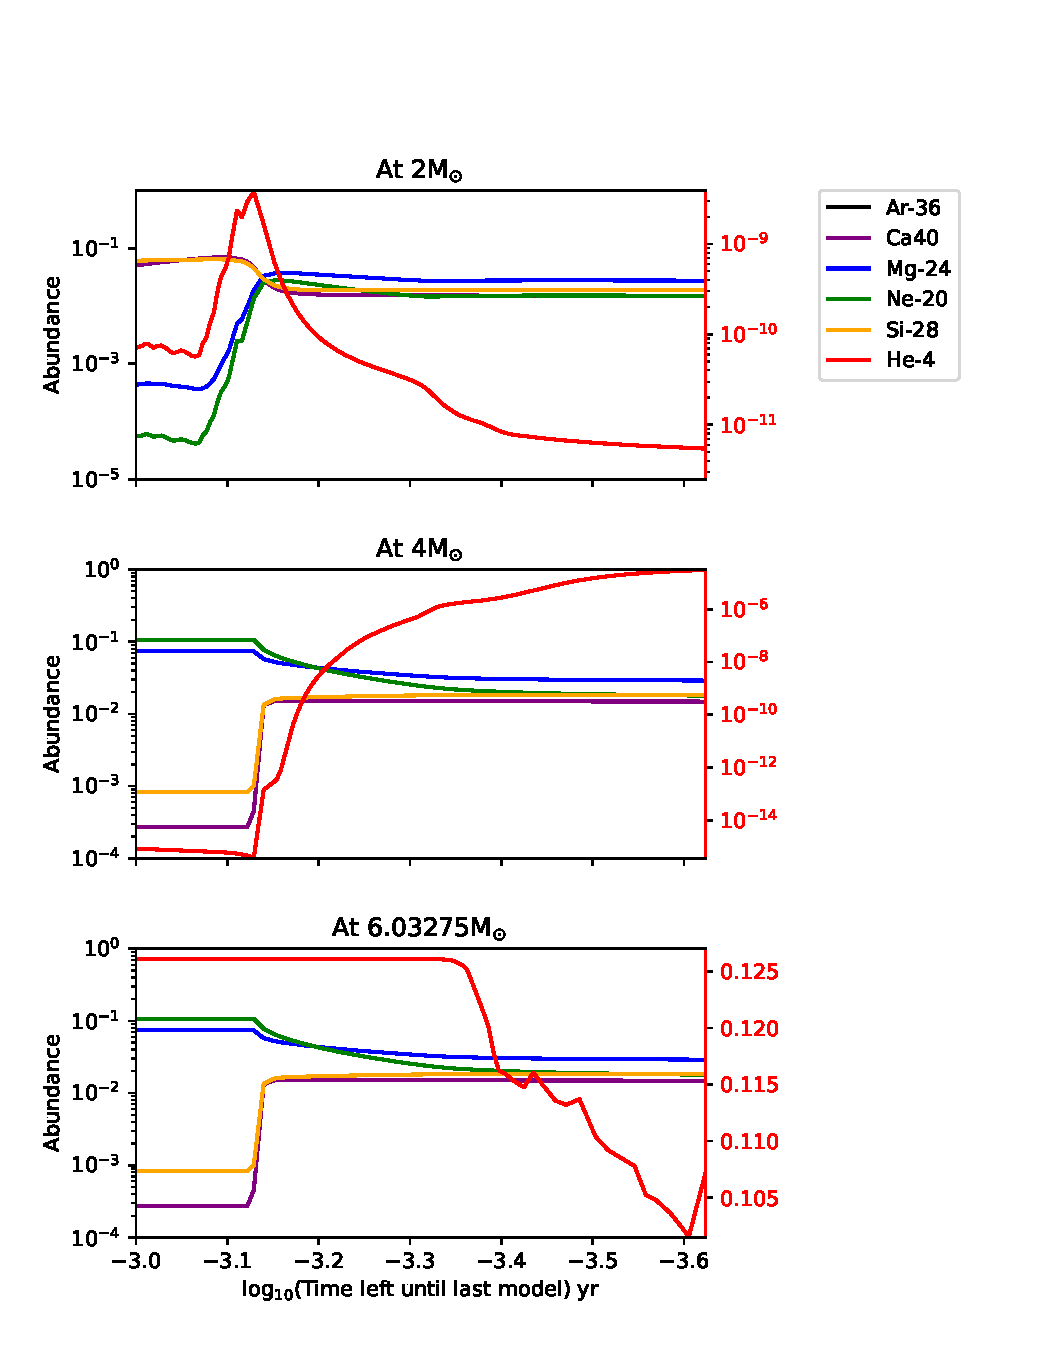
\includegraphics[width=0.7\linewidth]{Figures/HeMerger_Abundance.pdf}
    \caption{Isotopic abundances over time during the He shell merger event in a high resolution time-dependent convection run for three locations $\left(2M_{\odot},\ 4M_{\odot}, \ 6.03275M_{\odot}\right)$, where the right axis relates to He-4 abundance.}
    \label{fig:HeMerger_Abundance}
\end{center}
\end{figure*}